We now switch our attention and ask: given two (symmetric) random matrices $A_n, B_n \ensuremath{\in} \ensuremath{\bbR}^{n \ensuremath{\times} n}$, what are the distribution of the eigenvalues of $A_n+B_n$? If both $A_n$ and $B_n$ are Wigner matrices then so is their sum, so we are really interested in the case where one or both are not Wigner matrices (i.e., the distribution of the entries is not all the same or there is covariance between the entries).  The rather remarkable fact is that, as $n \ensuremath{\rightarrow} \ensuremath{\infty}$,  if we know the global distribution of $A_n$ and $B_n$, in the form of knowing the moments $\ensuremath{\bm{\mathrm{E}}} A_n^k$ and $\ensuremath{\bm{\mathrm{E}}} B_n^k$, under very broad conditions we can deduce the global distribution of $A_n+B_n$, in the form of knowing the moments $\ensuremath{\bm{\mathrm{E}}} (A_n+B_n)^k$, where again we use
\[
\ensuremath{\bm{\mathrm{E}}} f(A_n) := {1 \over n} \ensuremath{\bbE} \Tr f(A_n).
\]
In order to make sense of this, we think of the large $n$ limit of $A_n$ and $B_n$, a limit which does not exist in a traditional sense but we can formally write as $A$ and $B$, as an abstract algebra which behave simple rules.  For example, since $A_n$ and $B_n$ do not commute, neither do $A$ and $B$ ($AB \ensuremath{\neq} BA$). More specifically, $A$ and $B$ are  \emph{freely independent} non-commutative random variables, which is defined in terms of an expectation which we denote $\ensuremath{\bm{\mathrm{E}}}$, which satisfies
\[
    \ensuremath{\bm{\mathrm{E}}} f(A) = \lim_{n \ensuremath{\rightarrow} \ensuremath{\infty}} \ensuremath{\bm{\mathrm{E}}} f(A_n).
\]
(We have seen in the section on universality that even though $A_n$ itself doesn't really have a limit, $\ensuremath{\bm{\mathrm{E}}} f(A_n)$ will converge, and in particular behave like a semicircle.) By writing down the rules of $\ensuremath{\bm{\mathrm{E}}}$ we can deduce explicit formulae for the moments \ensuremath{\bm{\mathrm{E}}} (A+B)\^{}k, which will tell us the large $n$ behaviour of the eigenvalues of $A+B$. This can be thought of as a \emph{free convolution}, a non-commutative analogue of convolution. 

\textbf{Further Reading} \href{https://rolandspeicher.com/wp-content/uploads/2025/04/free-probability_v2.pdf}{Free Probability Theory} by Roland Speicher is an advanced introduction to the topic whilst \href{https://www.cambridge.org/core/services/aop-cambridge-core/content/view/B291B4E6728E10537C2406CE4C341923/S0962492904000236a.pdf/div-class-title-random-matrix-theory-div.pdf}{Random Matrix Theory} by Edelman and Rao gives a gentle but brief introduction.  Free Probability was introduced by \href{https://en.wikipedia.org/wiki/Dan-Virgil_Voiculescu}{Dan Voiculescu}, a prominent Berkeley operator theorist, in the 1980s. The connection with random matrix theory actually came much later in the early 1990s, as well as a detailed combinatorial description of Free Probability in terms of non-crossing partitions by Speicher.  It is a very modern and technical subject, and there is unfortunately limited material written for 1st year students beyond these notes. Rather exceptionally for an idea arising in pure mathematics, it has had an impact in a wide range of applications including wireless communication, quantum information, and most recently machine learning (where it has been used to study the transition from random-like behaviour of untrained networks to non-random behaviour of trained networks).

\section{Experimental observation of free convolutions}
We begin with an experimental observation of free convolution. Consider again a symmetric matrix $A_n \ensuremath{\in} \ensuremath{\bbR}^{n \ensuremath{\times} n}$  whose entries on and above the diagonal are iid random variables taking values $\ensuremath{\pm}1$ with equal probability. We saw in the previous chapter the global statistics are given by the semicircle. Now consider adding a diagonal matrix $D_n \ensuremath{\in} \ensuremath{\bbR}^{n \ensuremath{\times} n}$ with $\ensuremath{\pm}2$ on the diagonal with equal probability: what are the global statistics of $A_n + D_n$? We can explore this question numerically:


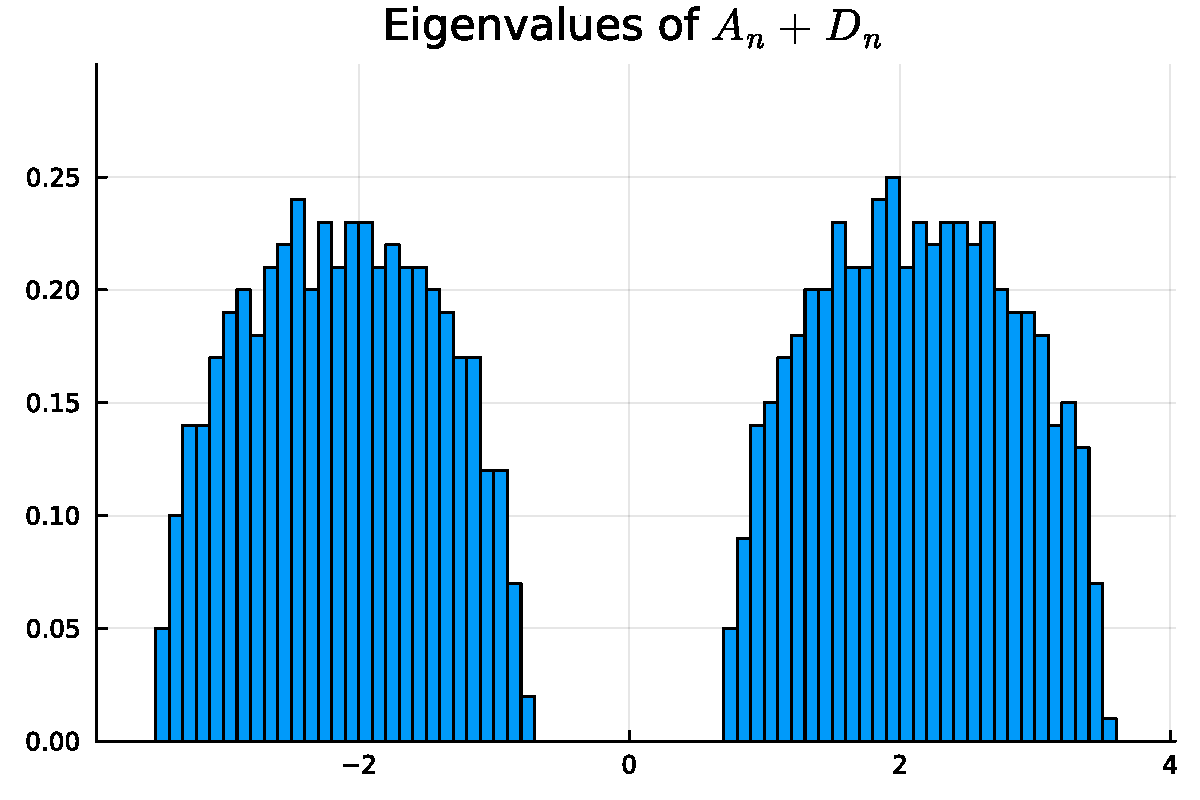
\includegraphics[width=0.6\linewidth,height=0.45\linewidth]{figures/III.FreeProbability_1_1.pdf}

We see that we get two semicircle-like distributions, surrounding \ensuremath{\pm}2. 

What's remarkable is this distribution only depends on the eigenvalues of $A_n$ and $D_n$. For example, consider the case where we same randomly $Q_n \ensuremath{\in} O(n)$, i.e., a random orthogonal matrix and define $B_n := Q_n D_n Q_n^\ensuremath{\top}$. This has exactly the same eigenvalues as $D_n$ itself. And when we add $A_n + B_n$ we get the exact same global statistics:


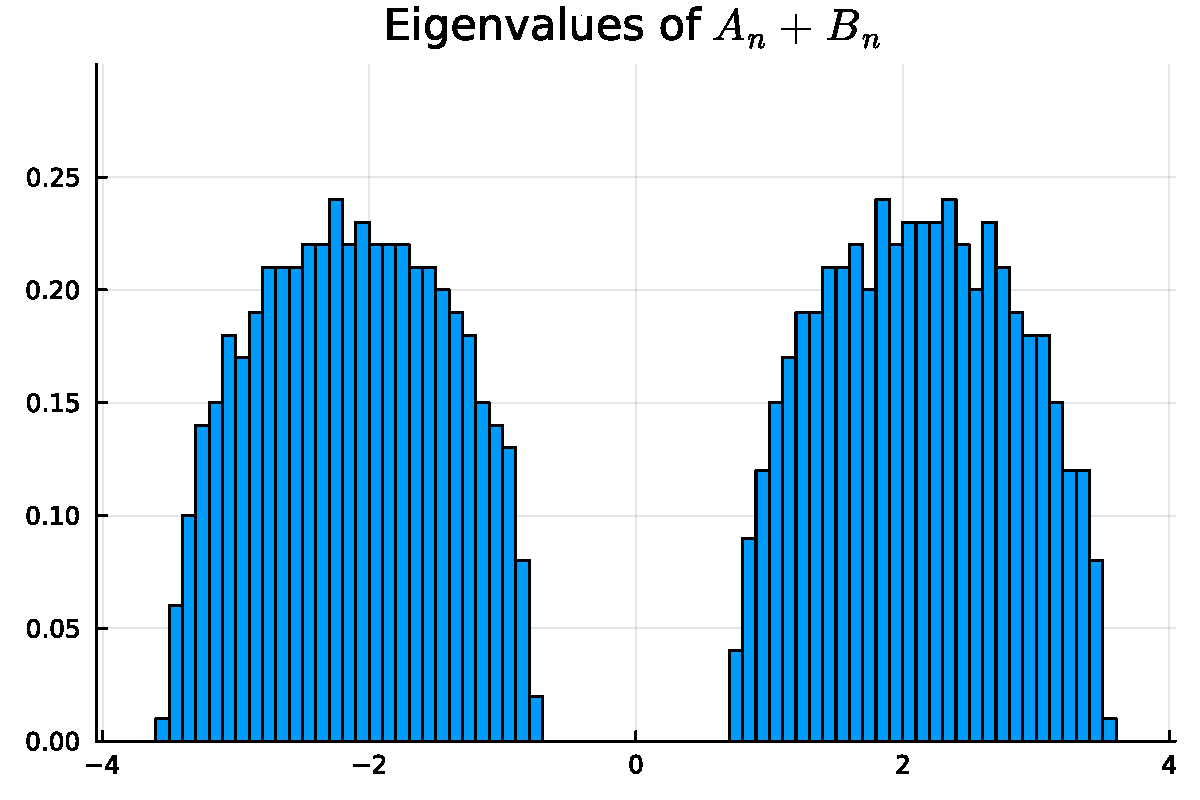
\includegraphics[width=0.6\linewidth,height=0.45\linewidth]{figures/III.FreeProbability_2_1.pdf}

This is a numerical demonstration of the fact that we can, under broad conditions, deduce the global eigenvalue statistics of $A_n + B_n$ from those of $A_n$ and $B_n$, and largely ignore the eigenvectors. To prove this we will again use the Method of Moments.

\section{Free random variables}
Since we aim to describe the behaviour of random matrices when the dimension becomes infinite, it's helpful to   put aside viewing $A$ and $B$ as matrices and instead think of them more abstractly as \emph{free random variables}, which are non-commutative random variables. With this convention, we will denote the identity element (the limit of the identity matrix $I_n$ as $n \ensuremath{\rightarrow} \ensuremath{\infty}$) as $1$.   Our free random variables expectation $\ensuremath{\bm{\mathrm{E}}}$ is no longer given explicitly in terms of a trace of a matrix, and instead we describe it more abstractly in terms of the properties it satisfies. 

With classical probability we have the feature that the expectations of the product of independent random variable equals the product of the expectation. More generally if $f$ and $g$ are polynomials and $X$ and $Y$ are independent we know:
\[
\ensuremath{\bbE}[f(X) g(Y)] = \ensuremath{\bbE}[f(X)] \ensuremath{\bbE}[g(Y)].
\]
We will see this particular property \emph{does} hold true for free probability. Where free probability differs to classical random variables is in alternating products: since $X$ and $Y$ are \emph{commutative}, if we have polynomials $f_1,\ensuremath{\ldots},f_n$ and $g_1,\ensuremath{\ldots},g_n$ then we clearly have
\[
\ensuremath{\bbE}[f_1(X) g_1(Y) \ensuremath{\cdots} f_n(X) g_n(Y)] = \ensuremath{\bbE}[f_1(X) \ensuremath{\cdots} f_n(X)] \ensuremath{\bbE}[g_1(Y) \ensuremath{\cdots} g_n(Y)],
\]
but this is no longer the case when $X$ and $Y$ do not commute.

Free probability comes from defining how these mixed moments behave in the case where the expectation vanishes:

\begin{definition}[free random variables] $A$ and $B$ are \emph{free random variables} equipped with an expectation $\ensuremath{\bm{\mathrm{E}}}$ if for all polynomials $f_1,\ensuremath{\ldots},f_n$ and $g_1,\ensuremath{\ldots},g_n$ such that $\ensuremath{\bm{\mathrm{E}}} f_k(A) = \ensuremath{\bm{\mathrm{E}}} g_k(B) = 0$ we have
\[
\ensuremath{\bm{\mathrm{E}}}[f_1(A) g_1(B) \ensuremath{\ldots} f_n(A) g_n(B)] = 0,
\]
where the identity element satisfies $\ensuremath{\bm{\mathrm{E}}} 1 = 1$. \end{definition}

We claim (without proof) that as $n \ensuremath{\rightarrow} \ensuremath{\infty}$ that ${1 \over n} \ensuremath{\bbE} \Tr$ behaves exactly like this for many families of random matrices. 

Note that we assume linearity: for constants $c,d$ we have
\[
\ensuremath{\bm{\mathrm{E}}}[c A + d B] = c \ensuremath{\bm{\mathrm{E}}}  A + d \ensuremath{\bm{\mathrm{E}}} B.
\]
It follows that (treating $\ensuremath{\bm{\mathrm{E}}}A^k$ as a constant)
\[
\ensuremath{\bm{\mathrm{E}}}[A^k - \ensuremath{\bm{\mathrm{E}}}A^k] =  \ensuremath{\bm{\mathrm{E}}} A^k - \ensuremath{\bm{\mathrm{E}}}A^k \ensuremath{\bm{\mathrm{E}}}1  = 0.
\]
This simple observation guarantees that if we know the moments $\ensuremath{\bm{\mathrm{E}}} A^k$ and $\ensuremath{\bm{\mathrm{E}}} B^k$ we can deduce the moments $\ensuremath{\bm{\mathrm{E}}}[A^k B^j]$. To see this, we first consider some of the low order cases. By subtracting off the free expectation of moments of $A$ and $B$ and treating $\ensuremath{\bm{\mathrm{E}}} A^k , \ensuremath{\bm{\mathrm{E}}}B^j$ as constants we deduce:
\meeq{
0 = \ensuremath{\bm{\mathrm{E}}}[(A^k-\ensuremath{\bm{\mathrm{E}}} A^k ) (B^j-\ensuremath{\bm{\mathrm{E}}}B^j )] =\ensuremath{\bm{\mathrm{E}}}[A^k B^j] - \ensuremath{\bm{\mathrm{E}}}[A^k \ensuremath{\bm{\mathrm{E}}}B^j]- \ensuremath{\bm{\mathrm{E}}}[\ensuremath{\bm{\mathrm{E}}}[A^k]B^j] + \ensuremath{\bm{\mathrm{E}}}[\ensuremath{\bm{\mathrm{E}}}A^k \ensuremath{\bm{\mathrm{E}}}B^j] \ccr
= \ensuremath{\bm{\mathrm{E}}}[A^k B^j] - \ensuremath{\bm{\mathrm{E}}}A^k \ensuremath{\bm{\mathrm{E}}}B^j \qquad \ensuremath{\Rightarrow} \qquad
\ensuremath{\bm{\mathrm{E}}}[A^k B^j] = \ensuremath{\bm{\mathrm{E}}}A^k \ensuremath{\bm{\mathrm{E}}}B^j
}
which matches the classical random variables formula $\ensuremath{\bbE}[A^k B^j] = \ensuremath{\bbE}A^k \ensuremath{\bbE}B^j$. This apparent consistency with classic random variables works for one mixed moment:
\meeq{
0 = \ensuremath{\bm{\mathrm{E}}}[(A-\ensuremath{\bm{\mathrm{E}}}A ) (B-\ensuremath{\bm{\mathrm{E}}}B )(A-\ensuremath{\bm{\mathrm{E}}}A )] \ccr
= 
\ensuremath{\bm{\mathrm{E}}}[ABA] -  \ensuremath{\bm{\mathrm{E}}}[AB\ensuremath{\bm{\mathrm{E}}}[A]] -\ensuremath{\bm{\mathrm{E}}}[A\ensuremath{\bm{\mathrm{E}}}[B]A] + \ensuremath{\bm{\mathrm{E}}}[A\ensuremath{\bm{\mathrm{E}}}[B]\ensuremath{\bm{\mathrm{E}}}[A]] \\
&\qquad - 
\ensuremath{\bm{\mathrm{E}}}[\ensuremath{\bm{\mathrm{E}}}[A]BA] + \ensuremath{\bm{\mathrm{E}}}[\ensuremath{\bm{\mathrm{E}}}[A]B\ensuremath{\bm{\mathrm{E}}}[A]] +  \ensuremath{\bm{\mathrm{E}}}[\ensuremath{\bm{\mathrm{E}}}[A]\ensuremath{\bm{\mathrm{E}}}[B]A]- \ensuremath{\bm{\mathrm{E}}}[\ensuremath{\bm{\mathrm{E}}}[A]\ensuremath{\bm{\mathrm{E}}}[B]\ensuremath{\bm{\mathrm{E}}}[A]]  \ccr
= 
\ensuremath{\bm{\mathrm{E}}}[ABA] - \ensuremath{\bm{\mathrm{E}}}A \underbrace{\ensuremath{\bm{\mathrm{E}}}[AB]}_{=\ensuremath{\bm{\mathrm{E}}}A\ensuremath{\bm{\mathrm{E}}}B}  - \ensuremath{\bm{\mathrm{E}}}B \ensuremath{\bm{\mathrm{E}}}A^2 -\ensuremath{\bm{\mathrm{E}}}A \underbrace{\ensuremath{\bm{\mathrm{E}}}[BA]}_{=\ensuremath{\bm{\mathrm{E}}}A\ensuremath{\bm{\mathrm{E}}}B}+2\ensuremath{\bm{\mathrm{E}}}[A]^2 \ensuremath{\bm{\mathrm{E}}}B \ccr
=
\ensuremath{\bm{\mathrm{E}}}[ABA] - \ensuremath{\bm{\mathrm{E}}}B \ensuremath{\bm{\mathrm{E}}}A^2\qquad \Rightarrow \ccr
\ensuremath{\bm{\mathrm{E}}}[ABA] = \ensuremath{\bm{\mathrm{E}}}A^2 \ensuremath{\bm{\mathrm{E}}}B.
}
But that's where the equivalence ends. In particular, consider:
\meeq{
0 = \ensuremath{\bm{\mathrm{E}}}[(A-\ensuremath{\bm{\mathrm{E}}}A ) (B-\ensuremath{\bm{\mathrm{E}}}B )(A-\ensuremath{\bm{\mathrm{E}}}A ) (B-\ensuremath{\bm{\mathrm{E}}}B ) ]\ccr
 = 
\ensuremath{\bm{\mathrm{E}}}[ABAB] - \underbrace{\ensuremath{\bm{\mathrm{E}}}[ABA]}_{=\ensuremath{\bm{\mathrm{E}}}A^2 \ensuremath{\bm{\mathrm{E}}}B}  \ensuremath{\bm{\mathrm{E}}}B -\ensuremath{\bm{\mathrm{E}}}A \underbrace{\ensuremath{\bm{\mathrm{E}}}[A B^2]}_{=\ensuremath{\bm{\mathrm{E}}}A \ensuremath{\bm{\mathrm{E}}}B^2}  + \underbrace{\ensuremath{\bm{\mathrm{E}}}[AB]}_{=\ensuremath{\bm{\mathrm{E}}}A\ensuremath{\bm{\mathrm{E}}}B} \ensuremath{\bm{\mathrm{E}}}A \ensuremath{\bm{\mathrm{E}}}B\\
&\qquad - \underbrace{\ensuremath{\bm{\mathrm{E}}}[A^2B]}_{=\ensuremath{\bm{\mathrm{E}}}A^2\ensuremath{\bm{\mathrm{E}}}B} \ensuremath{\bm{\mathrm{E}}}B + \ensuremath{\bm{\mathrm{E}}}A^2 \ensuremath{\bm{\mathrm{E}}}[B]^2 + \underbrace{\ensuremath{\bm{\mathrm{E}}}[A B]}_{=\ensuremath{\bm{\mathrm{E}}}A\ensuremath{\bm{\mathrm{E}}}[B]} \ensuremath{\bm{\mathrm{E}}}A \ensuremath{\bm{\mathrm{E}}}B - \ensuremath{\bm{\mathrm{E}}}[A]^2 \ensuremath{\bm{\mathrm{E}}}[B]^2\\
&\qquad - \ensuremath{\bm{\mathrm{E}}}[A] \underbrace{\ensuremath{\bm{\mathrm{E}}}[BA B]}_{=\ensuremath{\bm{\mathrm{E}}}A \ensuremath{\bm{\mathrm{E}}}B^2} + \ensuremath{\bm{\mathrm{E}}}A \ensuremath{\bm{\mathrm{E}}}B\underbrace{\ensuremath{\bm{\mathrm{E}}}[BA]}_{=\ensuremath{\bm{\mathrm{E}}}A\ensuremath{\bm{\mathrm{E}}}B}  + \ensuremath{\bm{\mathrm{E}}}[A]^2 \ensuremath{\bm{\mathrm{E}}}B^2 - \ensuremath{\bm{\mathrm{E}}}[A]^2 \ensuremath{\bm{\mathrm{E}}}[B]^2\\
&\qquad + \ensuremath{\bm{\mathrm{E}}}A \ensuremath{\bm{\mathrm{E}}}B \underbrace{\ensuremath{\bm{\mathrm{E}}}[AB]}_{=\ensuremath{\bm{\mathrm{E}}}A\ensuremath{\bm{\mathrm{E}}}B} - \ensuremath{\bm{\mathrm{E}}}[A]^2 \ensuremath{\bm{\mathrm{E}}}[B]^2  - \ensuremath{\bm{\mathrm{E}}}[A]^2 \ensuremath{\bm{\mathrm{E}}}[B]^2 +  \ensuremath{\bm{\mathrm{E}}}[A]^2 \ensuremath{\bm{\mathrm{E}}}[B]^2 \ccr
= \ensuremath{\bm{\mathrm{E}}}[ABAB] - \ensuremath{\bm{\mathrm{E}}}A^2 \ensuremath{\bm{\mathrm{E}}}[B]^2 - \ensuremath{\bm{\mathrm{E}}}[A]^2 \ensuremath{\bm{\mathrm{E}}}B^2 + \ensuremath{\bm{\mathrm{E}}}[A]^2 \ensuremath{\bm{\mathrm{E}}}[B]^2 \qquad \Rightarrow \ccr
\ensuremath{\bm{\mathrm{E}}}[ABAB] = \ensuremath{\bm{\mathrm{E}}}A^2 \ensuremath{\bm{\mathrm{E}}}[B]^2 + \ensuremath{\bm{\mathrm{E}}}[A]^2 \ensuremath{\bm{\mathrm{E}}}B^2 - \ensuremath{\bm{\mathrm{E}}}[A]^2 \ensuremath{\bm{\mathrm{E}}}[B]^2
}
which differs from the classical (commutative) case  where $\ensuremath{\bbE}[ABAB] = \ensuremath{\bbE}A^2 \ensuremath{\bbE}B^2$. Nevertheless, we can see the central theme emerging: $\ensuremath{\bm{\mathrm{E}}}[ABAB]$ is still given in terms of a function of the input moments $\ensuremath{\bm{\mathrm{E}}}A^k$ and $\ensuremath{\bm{\mathrm{E}}}B^j$:

\begin{lemma}[mixed moments] For $k_1,\ensuremath{\ldots},k_n$ and $j_1,\ensuremath{\ldots},j_n$ the mixed moments
\[
\ensuremath{\bm{\mathrm{E}}}[A^{k_1} B^{j_1} \ensuremath{\cdots} A^{k_n} B^{j_n}]
\]
can be expressed as functions of the moments
\[
\ensuremath{\bm{\mathrm{E}}}A, \ensuremath{\bm{\mathrm{E}}} A^2 \ensuremath{\ldots}, \ensuremath{\bm{\mathrm{E}}}A^{k_1 + \ensuremath{\cdots} + k_n}, \ensuremath{\bm{\mathrm{E}}}B, \ensuremath{\bm{\mathrm{E}}}B^2  \ensuremath{\ldots}, \ensuremath{\bm{\mathrm{E}}}B^{j_1 + \ensuremath{\cdots} + j_n}.
\]
\end{lemma}
\textbf{Proof} The proceeding example can be turned into a proof by induction. We leave this as a possible poster project. \ensuremath{\QED}

Unfortunately, there is no simple formula for the relationship between the moments of $A$ and $B$ and those of the mixed moments, but they can be derived systematically like we did for the first four moments. Note the cyclic property of trace we can be used to simplify some calculations because we have
\[
\ensuremath{\bm{\mathrm{E}}}[A^{k_1} B^{j_1} \ensuremath{\cdots} A^{k_n} B^{j_n}] = \ensuremath{\bm{\mathrm{E}}}[ B^{j_1} \ensuremath{\cdots} A^{k_n} B^{j_n} A^{k_1}] = 
\ensuremath{\bm{\mathrm{E}}}[B^{j_n} A^{k_1} B^{j_1} \ensuremath{\cdots} A^{k_n}].
\]
For example, we can deduce all moments up to degree 4 using the above calculations:
\meeq{
\ensuremath{\bm{\mathrm{E}}}[AB] = \ensuremath{\bm{\mathrm{E}}}[BA] = \ensuremath{\bm{\mathrm{E}}}A \ensuremath{\bm{\mathrm{E}}}B \ccr
\ensuremath{\bm{\mathrm{E}}}[ABA] =\ensuremath{\bm{\mathrm{E}}}[A^2 B]  =\ensuremath{\bm{\mathrm{E}}}[B A^2] = \ensuremath{\bm{\mathrm{E}}}A^2 \ensuremath{\bm{\mathrm{E}}}B \ccr
\ensuremath{\bm{\mathrm{E}}}[BAB] =\ensuremath{\bm{\mathrm{E}}}[B^2 A]  =\ensuremath{\bm{\mathrm{E}}}[A B^2] = \ensuremath{\bm{\mathrm{E}}}A \ensuremath{\bm{\mathrm{E}}}B^2 \ccr
\ensuremath{\bm{\mathrm{E}}}[A^2BA] = \ensuremath{\bm{\mathrm{E}}}[ABA^2] = \ensuremath{\bm{\mathrm{E}}}[A^3 B] = \ensuremath{\bm{\mathrm{E}}}[B A^3] = \ensuremath{\bm{\mathrm{E}}}A^3 \ensuremath{\bm{\mathrm{E}}} B \ccr
\ensuremath{\bm{\mathrm{E}}}[B^2AB] = \ensuremath{\bm{\mathrm{E}}}[BAB^2] = \ensuremath{\bm{\mathrm{E}}}[B^3 A] = \ensuremath{\bm{\mathrm{E}}}[A B^3] = \ensuremath{\bm{\mathrm{E}}}A \ensuremath{\bm{\mathrm{E}}} B^3 \ccr
\ensuremath{\bm{\mathrm{E}}}[A B^2 A] = \ensuremath{\bm{\mathrm{E}}}[B A^2 B] = \ensuremath{\bm{\mathrm{E}}}[A^2 B^2] = \ensuremath{\bm{\mathrm{E}}}[B^2 A^2] =  \ensuremath{\bm{\mathrm{E}}}A^2 \ensuremath{\bm{\mathrm{E}}} B^2 \ccr
\ensuremath{\bm{\mathrm{E}}}[BABA] = \ensuremath{\bm{\mathrm{E}}}[ABAB] = \ensuremath{\bm{\mathrm{E}}}A^2 \ensuremath{\bm{\mathrm{E}}}[B]^2 + \ensuremath{\bm{\mathrm{E}}}[A]^2 \ensuremath{\bm{\mathrm{E}}}B^2 - \ensuremath{\bm{\mathrm{E}}}[A]^2 \ensuremath{\bm{\mathrm{E}}}[B]^2.
}
Note that there $2^k$ moments of degree $k$ since each ``slot" can be either $A$ or $B$, and we can confirm we have all of them, when we include in the two trivial cases of $\ensuremath{\bm{\mathrm{E}}}A^k$ and $\ensuremath{\bm{\mathrm{E}}}B^k$. 

\section{Free convolution}
An implication of the previous lemma is that the expectation of all polynomials of $A$ and $B$ can be expressed in terms of the moments of $A$ and $B$. Note the moments of $A+B$ are polynomials in mixed moments, for example, here we walk through the first few examples using the explicit formul\ensuremath{\ae} for mixed moments (noting powers $(A+B)^k$ pick up every possible one of the $2^k$ mixed moments exactly once):
\meeq{
\ensuremath{\bm{\mathrm{E}}}[A+B] = \ensuremath{\bm{\mathrm{E}}}A+  \ensuremath{\bm{\mathrm{E}}} B \ccr
\ensuremath{\bm{\mathrm{E}}}[(A+B)^2] = \ensuremath{\bm{\mathrm{E}}}A^2 + \underbrace{\ensuremath{\bm{\mathrm{E}}}[AB]}_{=\ensuremath{\bm{\mathrm{E}}}A \ensuremath{\bm{\mathrm{E}}}B} + \underbrace{\ensuremath{\bm{\mathrm{E}}}[BA]}_{=\ensuremath{\bm{\mathrm{E}}}A \ensuremath{\bm{\mathrm{E}}}B} + \ensuremath{\bm{\mathrm{E}}}B^2 =  \ensuremath{\bm{\mathrm{E}}}A^2+ 2\ensuremath{\bm{\mathrm{E}}}A \ensuremath{\bm{\mathrm{E}}}B  + \ensuremath{\bm{\mathrm{E}}}B^2  \ccr
\ensuremath{\bm{\mathrm{E}}}[(A+B)^3] = \ensuremath{\bm{\mathrm{E}}}A^3  + \underbrace{\ensuremath{\bm{\mathrm{E}}}[A^2 B]}_{=\ensuremath{\bm{\mathrm{E}}}A^2 \ensuremath{\bm{\mathrm{E}}}B} + \underbrace{\ensuremath{\bm{\mathrm{E}}}[ABA]}_{=\ensuremath{\bm{\mathrm{E}}}A^2 \ensuremath{\bm{\mathrm{E}}}B} + \underbrace{\ensuremath{\bm{\mathrm{E}}}[AB^2]}_{=\ensuremath{\bm{\mathrm{E}}}A \ensuremath{\bm{\mathrm{E}}}B^2}  + \underbrace{\ensuremath{\bm{\mathrm{E}}}[BA^2]}_{=\ensuremath{\bm{\mathrm{E}}}A^2 \ensuremath{\bm{\mathrm{E}}}B}  + \underbrace{\ensuremath{\bm{\mathrm{E}}}[BAB]}_{=\ensuremath{\bm{\mathrm{E}}}A \ensuremath{\bm{\mathrm{E}}}B^2}+ \underbrace{\ensuremath{\bm{\mathrm{E}}}[B^2A]}_{=\ensuremath{\bm{\mathrm{E}}}A \ensuremath{\bm{\mathrm{E}}}B^2}+ \ensuremath{\bm{\mathrm{E}}}B^3 \ccr
 =  \ensuremath{\bm{\mathrm{E}}}A^3 + 3 \ensuremath{\bm{\mathrm{E}}} A^2 \ensuremath{\bm{\mathrm{E}}} B + 3 \ensuremath{\bm{\mathrm{E}}}A B^2 + \ensuremath{\bm{\mathrm{E}}}B^3 \ccr
\ensuremath{\bm{\mathrm{E}}}[(A+B)^4] = \ensuremath{\bm{\mathrm{E}}}A^4  + \underbrace{\ensuremath{\bm{\mathrm{E}}}[A^3 B]}_{=\ensuremath{\bm{\mathrm{E}}}A^3 \ensuremath{\bm{\mathrm{E}}}B} + \underbrace{\ensuremath{\bm{\mathrm{E}}}[A^2BA]}_{=\ensuremath{\bm{\mathrm{E}}}A^3 \ensuremath{\bm{\mathrm{E}}}B} + \underbrace{\ensuremath{\bm{\mathrm{E}}}[A^2 B^2]}_{=\ensuremath{\bm{\mathrm{E}}}A^2 \ensuremath{\bm{\mathrm{E}}}B^2}  + \underbrace{\ensuremath{\bm{\mathrm{E}}}[ABA^2]}_{=\ensuremath{\bm{\mathrm{E}}}A^3 \ensuremath{\bm{\mathrm{E}}}B}\\
&\qquad   + \underbrace{\ensuremath{\bm{\mathrm{E}}}[ABAB]}_{=\ensuremath{\bm{\mathrm{E}}}A^2 \ensuremath{\bm{\mathrm{E}}}[B]^2 + \ensuremath{\bm{\mathrm{E}}}[A]^2 \ensuremath{\bm{\mathrm{E}}}B^2 - \ensuremath{\bm{\mathrm{E}}}[A]^2 \ensuremath{\bm{\mathrm{E}}}[B]^2}+ \underbrace{\ensuremath{\bm{\mathrm{E}}}[AB^2A]}_{=\ensuremath{\bm{\mathrm{E}}}A^2 \ensuremath{\bm{\mathrm{E}}}B^2}\\
&\qquad  + \underbrace{\ensuremath{\bm{\mathrm{E}}}[AB^3]}_{=\ensuremath{\bm{\mathrm{E}}}A \ensuremath{\bm{\mathrm{E}}}B^3} + \underbrace{\ensuremath{\bm{\mathrm{E}}}[BA^3]}_{=\ensuremath{\bm{\mathrm{E}}}A^3 \ensuremath{\bm{\mathrm{E}}}B}+ \underbrace{\ensuremath{\bm{\mathrm{E}}}[BA^2B]}_{=\ensuremath{\bm{\mathrm{E}}}A^2 \ensuremath{\bm{\mathrm{E}}}B^2} + \underbrace{\ensuremath{\bm{\mathrm{E}}}[BABA]}_{=\ensuremath{\bm{\mathrm{E}}}A^2 \ensuremath{\bm{\mathrm{E}}}[B]^2 + \ensuremath{\bm{\mathrm{E}}}[A]^2 \ensuremath{\bm{\mathrm{E}}}B^2 - \ensuremath{\bm{\mathrm{E}}}[A]^2 \ensuremath{\bm{\mathrm{E}}}[B]^2} \\
&\qquad  + \underbrace{\ensuremath{\bm{\mathrm{E}}}[BAB^2]}_{=\ensuremath{\bm{\mathrm{E}}}A \ensuremath{\bm{\mathrm{E}}}B^3} + \underbrace{\ensuremath{\bm{\mathrm{E}}}[B^2A^2]}_{=\ensuremath{\bm{\mathrm{E}}}A^2 \ensuremath{\bm{\mathrm{E}}}B^2}+ \underbrace{\ensuremath{\bm{\mathrm{E}}}[B^2AB]}_{=\ensuremath{\bm{\mathrm{E}}}A \ensuremath{\bm{\mathrm{E}}}B^3} + \underbrace{\ensuremath{\bm{\mathrm{E}}}[B^3 A]}_{=\ensuremath{\bm{\mathrm{E}}}A \ensuremath{\bm{\mathrm{E}}}B^3}  + \ensuremath{\bm{\mathrm{E}}}B^4 \ccr
=  \ensuremath{\bm{\mathrm{E}}}A^4 + 4\ensuremath{\bm{\mathrm{E}}}A^3 \ensuremath{\bm{\mathrm{E}}}B + 4\ensuremath{\bm{\mathrm{E}}}A^2 \ensuremath{\bm{\mathrm{E}}}B^2 + 4\ensuremath{\bm{\mathrm{E}}}A \ensuremath{\bm{\mathrm{E}}}B^3 + \ensuremath{\bm{\mathrm{E}}}B^4 \\
&\qquad  + 2(\ensuremath{\bm{\mathrm{E}}}A^2 \ensuremath{\bm{\mathrm{E}}}[B]^2 + \ensuremath{\bm{\mathrm{E}}}[A]^2 \ensuremath{\bm{\mathrm{E}}}B^2 - \ensuremath{\bm{\mathrm{E}}}[A]^2 \ensuremath{\bm{\mathrm{E}}}[B]^2).
}
Note that up until the 4th moment the calculation is equivalent to classical convolution, and in particular the calcluation is an affine function of each of the ``input" moments. The 4th moment is where free convolution starts to differ, and the last term is a truely nonlinear function of the moments.  

Unfortunately there is no simple combinatorial formula for these expressions. But there is a miraculous equivalent way of constructing them. Consider the Stieltjes transform associated with the moments of $A$, i.e., the moment generating function of the form:
\[
G_A(z) := {1 \over z} + {\ensuremath{\bm{\mathrm{E}}} A \over z^2} + {\ensuremath{\bm{\mathrm{E}}} A^2  \over z^3} + \ensuremath{\cdots}.
\]
I like to think of this as a ``Taylor series around \ensuremath{\infty}"; actually, in a neighbourhood of \ensuremath{\infty} in the complex plane (hence the usage of $z$) but this is beyond what you have learned as 1st year students. Thus it is conceptually easier to recast this as a Taylor series around the origin via the transformation:
\[
\tilde{G}_A(z) := G_A(z^{-1}) = z + \ensuremath{\sum}_{k=2}^\ensuremath{\infty} \ensuremath{\bm{\mathrm{E}}} A^{k-1} z^k.
\]
Because its derivative at zero is nonzero (its 1) we know from the \emph{Inverse Function Theorem} that $\tilde{G}_A$ is invertible for small $z$, thus there exists a function $\tilde{G}_A^{-1}$ so that $\tilde{G}_A(\tilde{G}_A^{-1}(w)) = w$    which also has some Taylor series:
\[
\tilde{G}_A^{-1}(w) = w + \ensuremath{\sum}_{k=2}^\ensuremath{\infty} \tilde{r}_{A,k} w^k
\]
where $\tilde{r}_{A,k}$ are some functions of $\ensuremath{\bm{\mathrm{E}}} A^k$.  (One can actually deduce them systematically by matching terms!) We can thence deduce that $G_A$ itself has an inverse for small $w$ via:
\[
G_A^{-1}(w) := 1/\tilde{G}_A^{-1}(w) = {1 \over w} + {r_{A,2} \over w^2} + {r_{A,3} \over w^3} + \ensuremath{\cdots},
\]
where $r_{A,k}$ can be deduced from $\tilde{r}_{A,k}$, since we have 
\[
G_A(G_A^{-1}(w)) = \tilde{G}_A(1/G_A^{-1}(w)) = \tilde{G}_A(\tilde{G}_A^{-1}(w)) = w.
\]
We now define the \emph{R-transform}:
\[
R_A(w) := G_A^{-1}(w) - {1 \over w} = {r_{A,2} \over w^2} + {r_{A,3} \over w^3} + \ensuremath{\cdots}.
\]
The miraculous fact is that the R-transform of $A+B$ is given by the sum of the R-transforms of $A$ and $B$:
\[
R_{A+B}(z) = R_A(z) + R_B(z).
\]
Proving this is a very serious combinatorial problem connected to noncrossing partitions, which could be an excellent poster project.

\textbf{Example (adding two semicircles)} We conclude with an example where we can do everything explicitly. Suppose $A$ and $B$ are the large $n$ limits of two independent Wigner ensembles. We know that $A+B$ is also the large $n$ limit of a Wigner ensemble (but with double the variance) so will also have a semicircle eigenvalue distribution. How do we see this fact come out of free convolution? In this case the moments are identical:
\[
\ensuremath{\bm{\mathrm{E}}} A^k = \ensuremath{\bm{\mathrm{E}}} B^k = \begin{cases} C_{k/2} & k\hbox{ even} \\
    0 & k\hbox{ odd} \end{cases}.
\]
We therefore have
\[
\tilde{G}_A(z) \ensuremath{\equiv} \tilde{G}_B(z) = z + \ensuremath{\sum}_{k=2}^\ensuremath{\infty} \ensuremath{\bm{\mathrm{E}}} A^{k-1} z^k = C_0 z + C_1 z^3 + C_2 z^5 + \ensuremath{\cdots}.
\]
Now comes the key trick: we can use the recurrence for Catalan numbers to deduce
\meeq{
\tilde{G}_A(z)^2 = z^2 \br[C_0^2 + (C_0 C_1 + C_1 C_0) z^2 + (C_0 C_2 + C_1 C_1 + C_1 C_2) z^4 + \ensuremath{\cdots}]\ccr
 = z^2 \ensuremath{\sum}_{k=0}^\ensuremath{\infty} z^{2k} \underbrace{\ensuremath{\sum}_{j=0}^k C_j C_{k-j}}_{= C_{k+1}} = 
C_1 z^2 + C_2 z^4 + C_3 z^6 \ensuremath{\cdots} = {\tilde{G}_A(z) \over z} - 1.
}
We can now use the quadratic formula to deduce
\[
\tilde{G}_A(z) = {z^{-1} \ensuremath{\pm} \sqrt{z^{-2} -4} \over 2} = {1 - \sqrt{1 -4 z^2} \over 2 z}
\]
where the negative sign is chosen so that $\tilde{G}_A$ does not blow up at $0$ (by L'Hopital's rule).  A consequence of this is that:
\[
G_A(z) = {z - \sqrt{z^2 -4} \over 2}
\]
which \emph{does} decay as $z \ensuremath{\rightarrow} \ensuremath{\infty}$ (Why?). 

Now we want to find the functional inverse by solving:
\meeq{
w = G_A(z) = {z - \sqrt{z^2 -4} \over 2}\qquad  \ensuremath{\Rightarrow} \qquad  (2w-z)^2 = z^2 - 4 \\
 &\ensuremath{\Rightarrow} \qquad -4wz + 4w^2 = -4 \qquad  \ensuremath{\Rightarrow} \qquad  z = {1 \over w} +w,
}
i.e. we have
\[
G_A^{-1}(w) = {1 \over w} +w.
\]
Thus the R-transform is particularly simple:
\[
R_A(w) = G_A^{-1}(w) - {1 \over w} = w
\]
which is also the R-transform for $B$. Thus we know
\[
R_{A+B}(w) = 2 w \qquad \ensuremath{\Rightarrow} \qquad G_{A+B}^{-1}(w) = {1 \over w} + 2w.
\]
We can now solve
\[
z = {1 \over w} + 2w \qquad \Rightarrow \qquad zw = 1 + 2w^2 \qquad \Rightarrow \qquad w = {z - \sqrt{z^2 - 8} \over 4}
\]
i.e. we know that
\[
G_{A+B}(z) = {z - \sqrt{z^2 - 8} \over 4}.
\]
We leave the final step of finding the moments and distribution as a possible poster project. But actually from this formula we can do an educated guess: since the square-root vanishes at $z = \ensuremath{\pm}\sqrt{8} = \ensuremath{\pm}2 \sqrt{2}$ we can guess that the distribution is a semicircle with the same endpoints, i.e.,
\[
{\sqrt{8 - x^2} \over 4 \ensuremath{\pi}}.
\]
\section{Poster projects}
Here are some ideas for poster projects related to free probability:

\begin{itemize}
\item[1. ] Investigate why two Wigner ensembles $A_n$ and $B_n$ follow the rules of free probability as $n \ensuremath{\rightarrow} \ensuremath{\infty}$.


\item[2. ] Understanding all free probability operations including multiplication and truncation (e.g., the limit of $A_n[1:n-m,1:n-m]$). These operations can also be reduced to simple functions of the input moments, and one could walk through low orders.


\item[3. ] Explore the Free Central Limit Theorem either mathematically or experimentally,  where $A_1 + \ensuremath{\cdots} + A_n$ tends to a semicircle when $A_k$ are free and independent.


\item[4. ] Complete the derivation of the addition of two semicircles and explore further examples like the Marchenko\ensuremath{\endash}Pastur distribution.


\item[5. ] Do additions and multiplications of random matrices still exhibit universality in local statistics?

\end{itemize}

